\subsection{Specific Aim 3: Dynamics of self-assembly by HAP under an external flow/field}
\label{subsec:specific_aim_3}

\subsubsection{Vesicles in background flows}
Numerically solving the Stokes and screened Laplace system~\eqref{SL}
and~\eqref{eq:stokes} is nontrivial, and we will develop efficient,
robust, high-order in time and space algorithms suited to the problem.
The challenges are: {\bf (1)} the equations express a two-way coupling.
This means that the flow changes the shape of the suspended particles,
and in return the geometry-dependent hydrophobic stresses impart a force
on the flow. {\bf (2)} The inputs to the Stokes equations are particle
configurations, forces, and torques. The outputs are the rigid body
translation and angular velocities used to update the particle positions
(see Figure~\ref{fig:flow_map}). Although the underlying equations are
linear, the overall problem is highly nonlinear because the domain is
constantly changing. {\bf (3)} Self-assembly causes the particles to
come into close contact. As a result, an exceptional spatial accuracy is
required to resolve the fields between adjacent particles. Finally, the
physically relevant elastic properties of bilayer become apparent at
large length scales and for large particle-numbers, which increases the
computational complexity of our simulations. 

We include a background flow by replacing the third equation in
\eqref{eq:stokes} with the condition $(\mathbf{u} -
\mathbf{u}_{\infty})(\mathbf{x}) \to \mathbf{0}$ as $|\mathbf{x}| \to
\infty$. To incorporate the far-field flow, we use the representation 
\begin{align}
\label{PowerMiranda}
  {\bf u} = {\bf u}_{\infty} + K\boldsymbol{\eta} + 
    \sum_{i=1}^N S(\cdot, {\bf a}_i) {\bf F}_i + 
                 R(\cdot, {\bf a}_i) {\bf G}_i.
\end{align}
where $S$ and $R$ are stokeslets and rotlets supported at the respective
particle centers and $K\boldsymbol{eta}$ is a layer potential for the
unknown density function $\boldsymbol{\eta}.$ The
representation~\eqref{PowerMiranda} automatically satisfies all
equations, with the exception of the rigid motion conditions. The rigid
motion conditions follow by requiring the viscous stress vanishes across
the particle boundaries.

%\begin{wrapfigure}[13]{r}{0.30\textwidth}
%\centerline{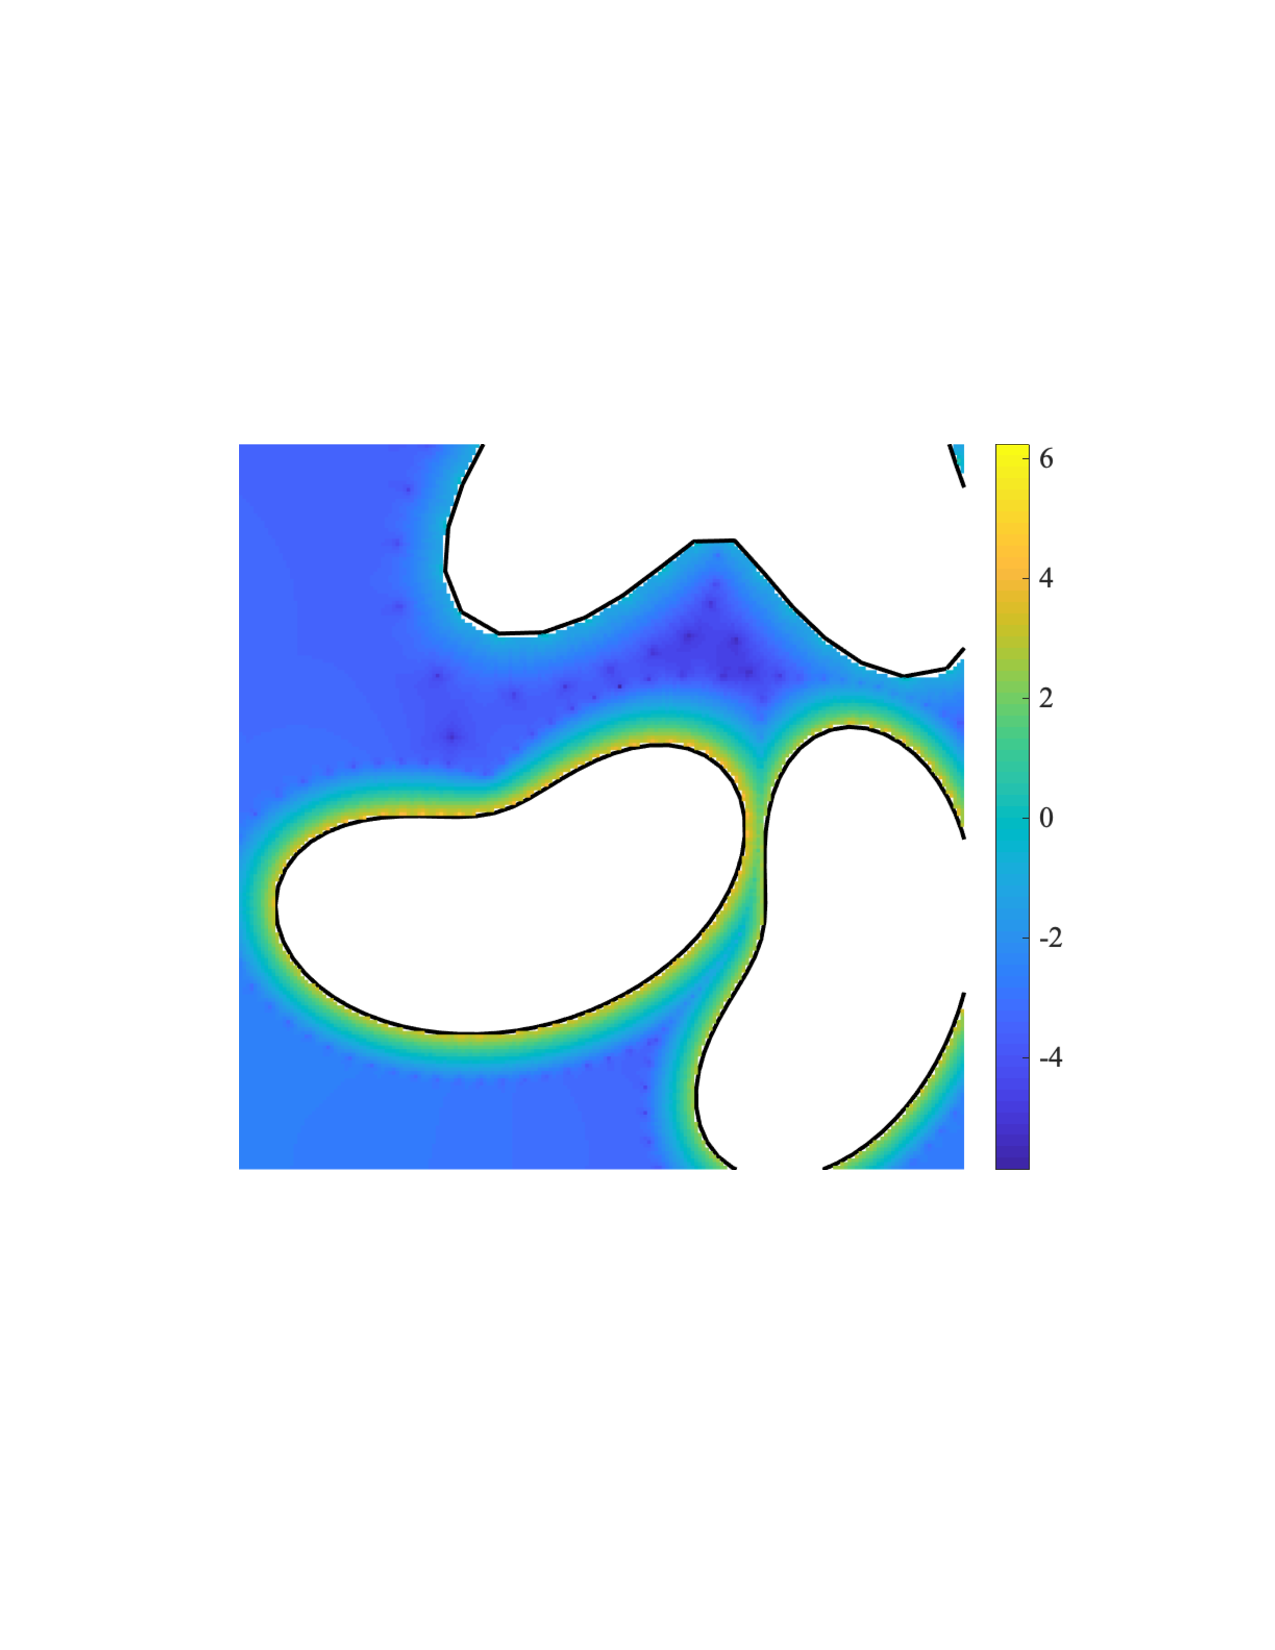
\includegraphics[width=0.30\textwidth]{figures/BIError.pdf}}
%  \vspace{-8pt}
%\caption{
%\label{fig:bierror}  
%\footnotesize The false color map shows how numerical quadrature of
%  layer potentials loses accuracy near the particle boundaries.  The
%  color bar is for $\log_{10}.$}
%\end{wrapfigure}

We will compare the behavior of our particle-based vesicles in Stokes
flow to well-established models that enforce area incompressibility and
volume conservation in vesicle membrane
dynamics~\cite{torres-sanchez_millan_arroyo_2019,
mahapatra_saintillan_rangamani_2020, Steigmann99, C6SM02452A}. Our
preliminary results show that the particle-based bilayers have the same
large area modulus as real lipid bilayer membranes, so we expect
realistic results from our flow simulations. Under moderate shear rates,
the vesicle elongates and takes on the tank-treading elliptical shape.
We can directly check for area compressibility conservation properties
from the particle simulation by tracking the change in area density of
the midplane as a function of shear flow rate, along with evaluating the
tangential divergence of the velocity.


Bilayer membranes have a small permeability to water
\cite{323e9a2f0c58487ea82518d7a1f96485}, and modelers often assume a
vesicle membrane that conserves volume. In our particle-based approach,
water motion across the bilayer is limited by the size of the gaps
between the particles, which is an artifact of coarse-graining.  Making
these gaps smaller comes at the expense of numerical accuracy, and we
will assess if there is a reasonable trade-off between approximate
volume conservation and simulation complexity. 



Finally, the particle-based vesicle bilayers have two distinct leaflets
consisting of the particles in contact with the vesicle interior, and
those in contact with the surrounding fluid. Since there is a nonzero
separation between these layers, an important effect we observe is that
the leaflets slide against one another under shear flow.  This implies
that part of the viscous dissipation in the aqueous phase is enhanced by
intermonolayer friction~\cite{SHKULIPA2005823, ShkulipaThesis}.
Intermonolayer slip enters zero-thickness membrane models as a velocity
jump boundary condition and leads to multiple solution
states~\cite{schwalbe_vlahovska_miksis_2010}.  In the present proposal,
intermonolayer slip is an artifact of monolayer independence  and we can
control for slip as a function of shear rate, vesicle diameter, and
particle geometry.

\subsubsection{Effects of electric fields on the dynamic self-assembly}




